\documentclass{scrartcl}
\usepackage{listings}
\usepackage{graphicx}
\usepackage[toc,page]{appendix}
\usepackage[utf8]{inputenc}
\usepackage{caption}
\usepackage{hyperref}
%\usepackage{math}

\usepackage{listings}
%\usepackage{fontspec}
%\DeclareFontShape{OT1}{cmtt}{bx}{n}{<5><6><7><8><9><10><10.95><12><14.4><17.28><20.74><24.88>cmttb10}{}

\author{Christophe Quignon}
\date{29.03.2014}
\title{Autonomous Mobile Robots Homework}
\begin{document}
\maketitle

\section{Give convincing estimates about the size of the state space used by the Deutsche Bahn App. This mean you should give a comprehensive calculation about how you reached your estimate. You base your estimates on public data available on the web.}
In 2012, the openPlanB iniciative scraped the "Kursbuch" off the DB which contained all trains, trainstations and connections in germany. The data was published \href{https://dl.dropbox.com/s/xonu0zy4wds5oua/openPlanB_\%20ODbL1.0_2012-09-04.torrent?dl=1}{as a torrent} and commented on their website \href{http://openplanb.tumblr.com/post/30878899005/die-ersten-fahrplandaten}{openplanb.tumblr.com}. As one can see in Figure \ref{viz} and look up in the published file, the search space with over 300.000 train stations and over 1 million trains, busses etc is immens.\\
Lets assume that the connectedness of the train stations follow a power law such that only a few stations (like cologne and bonn) are connectet to many other stations and the most are only connected to the station in front and behind them as it is the case in rural areas. By that I'd assume an average connectedness or branching factor of 3.\\
By that we have d = 300.000 and b = 3. Therefore the search space $d^{b}$ is $3^{300.000}$ whis is aproximately $10^{100.000}$ which is number with with 100.001 digits.

\begin{figure}
\center
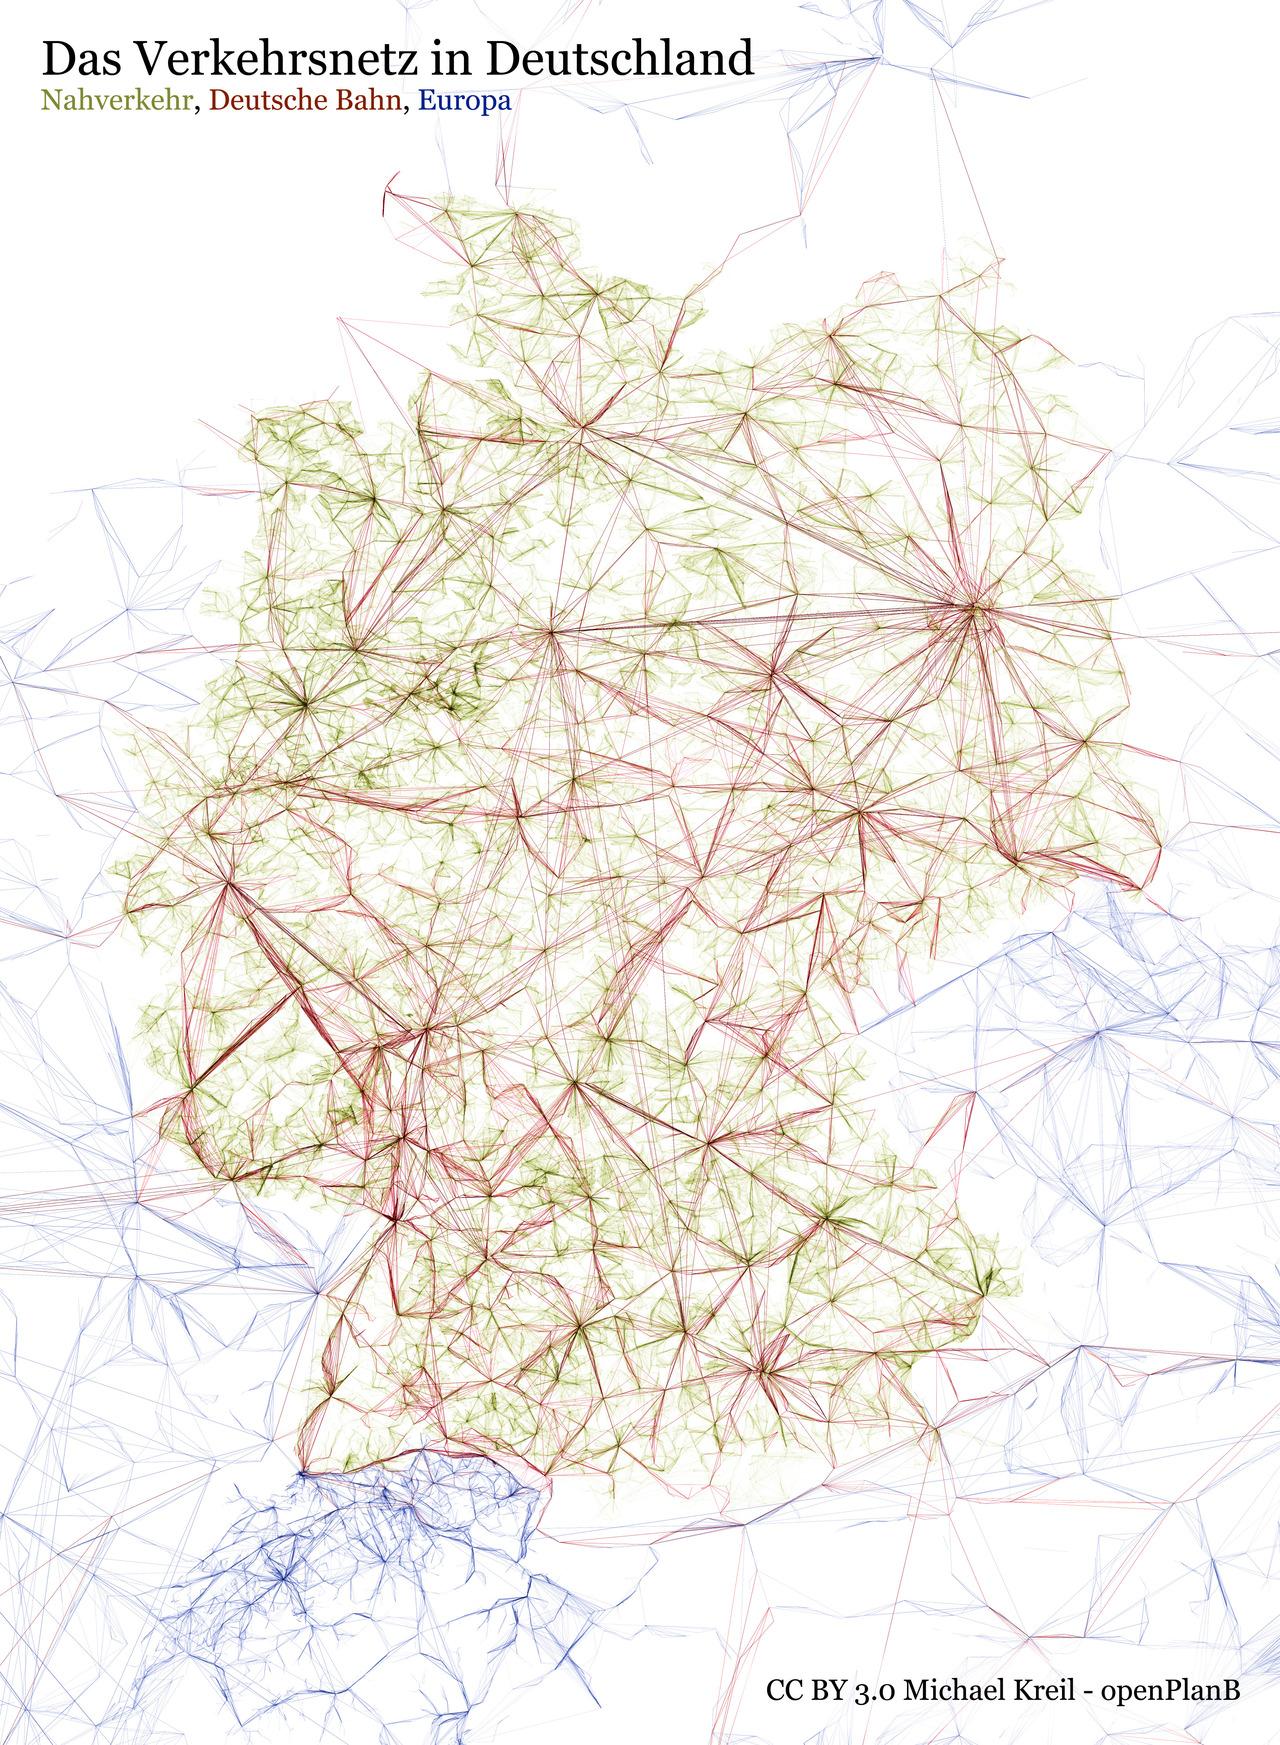
\includegraphics[width=16cm]{img/openDBviz.jpg}
\caption{Visualisation of the openplanB Data.}
\label{viz}
\end{figure}

\newpage
\begin{appendices} 

\section*{search.py}
\lstinputlisting{../src/astar.py}
\end{appendices}

\end{document}